\section{РЕАЛИЗАЦИЯ CLASS-BASED WFQ В ЯДРЕ LINUX}

	\subsection{Описание устройства подсистемы планировки в ядре Linux}

	В операционной системе Linux
	дисциплина обслуживания, обозначаемая термином qdisc, используется
	для выбора пакетов из выходящей очереди для отправки на выходной интерфейс.
	Схема движения пакета приведена на Рисунке~\ref{pic:flow}. Выходная очередь
	обозначена термином egress; именно на этом этапе следования пакета
	и работает механизм qdisc.\cite{lartc}

    \begin{figure}[ht!]
        \center
        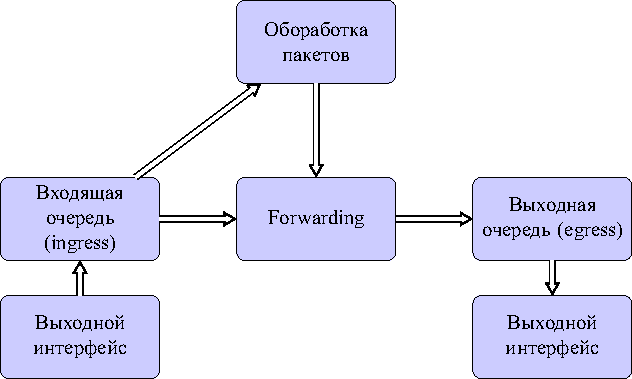
\includegraphics[scale=1.3]{pdfimages/qdisc.pdf}
        \caption{Схема движения пакета в системе Linux\cite{tcpip}. Красным отмечена стадия, в которой
				 работает механизм контроля качества обслуживания.}
		\label{pic:flow}
    \end{figure}

	В общем случае, дисциплина обслуживания --- это чёрный ящик, который может
	принимать поток пакетов и выпускать пакеты,
	когда устройство
	готово к отправке, в порядка и во время, определёнными спрятанным в ящике
	алгоритмом. В ядре Linux дисциплины обслуживания представляются в качестве
	модулей ядра, которые реализуют предоставляемый ядром интерфейс.

	Linux поддерживает классовые и бесклассовые дисциплины обслуживания. Примером
	бесклассовой дисциплины служит pfifo\_fast, классовой --- htb.\cite{lartc}

	Классы представляют собой отдельные сущности в иерархии основной дисциплины.
	Если структура представляет собой дерево, то в классах-узлах могут содержаться
	фильтры, которые определят пакет в нужный класс-потомок. В классах-листьях
	непосредственно располагаются очереди, которые управляются внутренней дисциплиной
	обслуживания. По умолчанию это pfifo\_fast, но можно назначить другие. 

	Каждый интерфейс имеет корневую дисциплину, которой
	назначается идентификатор (handle), который используется для обращения к дисциплине.
	Этот идентификатор состоит из двух частей: мажорной (MAJ) и минорной (MIN); мажорная
	часть определяет родителя, минорная --- непосредственно класс. На Рисунке~\ref{pic:clheirh}
	представлен пример иерархии.

	\begin{figure}[ht!]
		\centering
		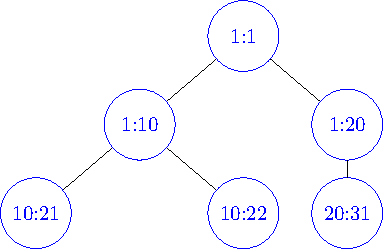
\includegraphics[scale=1.3]{./pdfimages/class_hierh.pdf}
		\caption{Схема классовой иерархии с использованием идентификаторов MAJ:MIN}
		\label{pic:clheirh}
	\end{figure}

	Идентификатор класса называется classid (к примеру, 1:10),
	а идентификатор его родителя --- parenid (1:1 для классов 1:10 и 1:20). По этим
	идентификаторам происходит поиск нужного класса внутри дисциплины.

	Такая иерархия позволяет организовать гибкую систему классификации с набором классов
	и их подклассов, пакеты в которые назначаются фильтрами, которые предоставляются ядром.

	\subsection{Интерфейс управления трафиком}

	В Linux управление трафиком осуществляется с помощью подсистемы Traffic Control,
	которая предоставляет пользовательский интерфейс с помощью утилиты {tc}.
	{tc} --- это пользовательская программа, которая позволяет настраивать
	дисциплины обслуживания в Linux. Она использует Netlink в качестве
	коммуникационного канала для взаимодействия между пользовательским
	пространством и пространством ядра. {tc} добавляет новые дисциплины
	обслуживания, классы трафика, фильтры и предоставляет команды для
	управление всеми обозначенными объектами.\cite{tcpip}

	{tc} предоставляет интерфейс для дисциплины обслуживания,
	представленный структурой \lstinline{struct qdisc_util}, которая
	описывает функции для отправления команд и соответствующих параметров ядру
	и вывода сообщений о настройки дисциплины, списках классов и их настройки, а
	также статистику от ядра. Сообщение, помимо общей информации для подсистемы,
	содержит специфичную для дисциплины структуру с опциями, описываемую
	в заголовке ядра {pkt\_sched.h}:
	\begin{itemize}
		\item структура \lstinline{struct tc_cbwfq_glob} определяет глобальные настройки
			  дисциплины обслуживания; структура передаётся по Netlink к модулю дисциплины
			  при инициализации и изменении настроек;
		\item структура \lstinline{struct tc_cbwfq_copt} определяет настройку
			  класса и используется при добавлении или изменения класса.
	\end{itemize}

	Патч для заголовка в Приложении А.

	Для назначения новой дисциплины обслуживания на интерфейс используется
	команда ``\lstinline{tc qdisc add}''  системными параметрами (к примеру, название
	интерфейса), названием дисциплины и её локальными параметрами, которые
	определяются и обрабатываются в модуле дисциплины для утилиты {tc}. 
	Для внесения изенений и удаления используются соответственно ``\lstinline{tc change}''
	и  ``\lstinline{tc delete}''.

	Опции для настройки дисциплины обслуживания:
	\begin{itemize}
		\item ``\lstinline{bandwidth}''---- пропускная способность B канала;
		\item ``\lstinline{default}''---- ключевое слово, определяющее, что далее пойдёт
									 настройка класса по умолчанию; опции те же самые, что
									 и при настройке класса.  
	\end{itemize}

	Для классовых дисциплин используется команда  ``\lstinline{tc class}'' с под командами
	 ``\lstinline{add}'',  ``\lstinline{change}'' и так далее. Классы обычно имеют параметры,
	отличные от параметров всей дисциплины обслуживания, поэтому нуждаются в отдельной
	структуре данных и функции обработчике.

	Опции для настройки класса:
	\begin{itemize}
		\item ``\lstinline{rate}''---- минимальная пропускная способность для класса;
											  задаётся в единицах скорости (Mbps, Kbps, bps) или в процентах
											  от размера канала (при использовании ключевого слова  ``\lstinline{percent}'');
		\item ``\lstinline{limit}''---- максимальное число пакетов в очереди.
	\end{itemize}

	Модуль для утилиты {tc} и ядра Linux, обеспечивающие взаимодействие между
	пользовательским пространством и дисциплиной представлен в Приложении Б. 

	\subsection{Описание интерфейса}

	API ядра для подсистемы qdisc предоставляет две функции: \lstinline{register_qdisc(struct Qdisc_ops *ops)}
	и обратную --- \lstinline{unregister_qdisc(struct Qdisc_ops *ops)}, которые регистрируют
	и разрегистрируют дисциплину обслуживания на интерфейсе. Важно отметить, что обе эти
	функции принимают в качестве аргумента структуру \lstinline{struct Qdisc_ops},
	которая явным образом идентифицирует дисциплину обслуживания в ядре.

	Структура \lstinline{struct Qdisc_ops} помимо метаинформации (в виде наименования дисциплины)
	содержит указатели на функции, которые должен реализовывать модуль дисциплины обслуживания
	для работы в ядре. Если не реализовать некоторые функции,
	то ядро в некоторых случаях попробует использовать функции по умолчанию, однако
	для особенно важных (к примеру, изменение конфигурации дисциплины или класса)
	сообщит пользователю, что операция не реализована.

	Поля структуры \lstinline{Qdisc_ops} представляют собой указатели на функции 
	представленными ниже сигнатурами.
	\begin{itemize}
		\item \lstinline{enqueue}\\
   		    \lstinline{int enqueue(struct sk_buff *skb, struct Qdisc *sch, struct sk_buff **to_free);} \\
			Функкция добавляет пакет в очередь. Если пакет был отброшен, функция
			возвращает код ошибки, говорящий о том, был отброшен пришедший пакет или
			иной, чьё место занял новый.
		\item \lstinline{dequeue}\\
			\lstinline{struct sk_buff *dequeue(struct Qdisc *sch);} \\
			Функция, возвращающая пакет из очереди на отправку. Дисциплина
			может не передавать пакет при вызове этой функции по решению
			алгоритма, в таком случае вернув нулевой указатель; 
			однако то же значение алгоритм возвращает в случае, если очередь
			пуста, поэтому в таком случае дополнительно проверяется длина
			очереди.
		\item \lstinline{peek}\\
			\lstinline{struct sk_buff *peek(struct Qdisc *sch);}\\
			Функция возвращает пакет из очереди на отправку, не удаляя его из реальной очереди,
			как это делает функция \lstinline{dequeue}.
		\item \lstinline{init}\\
			  \lstinline{int init(struct Qdisc *sch, struct nlattr *arg);}\\
			  Функция инициализирует вновь созданный экземпляр дисциплины обслуживания {sch}.
			  Вторым аргументом функции является конфигурация дисциплины обслуживания, передаваемая
			  в ядро с помощью подсистемы Netlink.
		\item \lstinline{change}\\
			  \lstinline{int change(struct Qdisc *sch, struct nlattr *arg);}\\
			  Функция изменяет текущие настройки дисциплины обслуживания. 
		\item \lstinline{dump}\\
			  \lstinline{int dump(struct Qdisc *sch, struct sk_buff *skb);}\\
			  Функция отправляет по Netlink статистику дисциплины обслуживания.
	\end{itemize}

	Также структура содержит указатель на \lstinline{struct Qdisc_class_ops},
	которая описывает указатели функции исключительно для классовых дисциплин.
	Ниже приведены наиболее важные сигнатуры и их описания.
	\begin{itemize}
		\item \lstinline{find}\\
			\lstinline{unsinged long find(struct Qdisc *sch, u32 classid);}\\
			Функция возвращает приведённый к \lstinline{unsinged long} адресс класса по его идентификатору (\lstinline{classid}).
		\item \lstinline{change} \\
			\lstinline{int change(struct Qdisc *sch, u32 classid, u32 parentid, struct nlattr *attr, unsinged long *arg);}\\
			Функция используется для изменения и добавления новых классов в иерархию классов. 
		\item \lstinline{tcf_block}, \lstinline{bind_tcf}, \lstinline{unbind_tcf}\\
			В данном случае, описание сигнатур не даст какой-либо значимой информации; практически
			для всех дисциплин обслуживания они идентичны. Эти функции предназначаются для работы
			системы фильтрации.
		\item \lstinline{dump_class}\\
			\lstinline{int dump_class(struct Qdisc *sch, unsinged long cl, struct sk_buff *skb, struct tcmsg *tcm);} \\
			Функция предназначается для передачи по Netlink информации о классе и дополнительной статистики, собранной
			во время функционирования класса.
	\end{itemize}

	Для классовых дисциплин, помимо описанного, реализуют классификацию пакетов, которая
	определяет класс, куда попадаёт пакет. Классификация обычно выражается в функции \lstinline{classify},
	которая вызывается при добавлении пакета в очередь (функция \lstinline{enqueue}) определяет, какому классу
	 принадлежит пакет, и возвращает указатель на этот класс.
	Экземпляр структур для дисциплины обслуживания CBWFQ приведён в патче, представленном в Приложении В.

	\subsection{Алгоритм CBWFQ}

		Реализация CBWFQ требует:
		\begin{itemize}
			\item вычисление порядкового номера для каждого пакета в очередях и содержание глобального счётчика циклов;
			\item поддержку классов и классовых операций;
			\item фильтрацию для классификации трафика по классам.
		\end{itemize}

		\subsubsection{Структуры хранения данных Class-Based WFQ}
	
			Обычно классовые дисциплины обслуживания содержат две основные структуры:
			для описания непосредственно дисциплины и для описания класса.  
			Структура дисциплины содержит в себе данные, которые описывают всю дисциплину:
			это могут быть структура данных с классами (в виде списка или дерева),
			ограничения на очереди, статистика по всей дисциплине и так далее.
			Структура класса, соответственно, содержит непосредственно очередь и описывающие
			класс параметры.

			Описание полей структуры дисциплины обслуживания \lstinline{struct cbwfq_sched_data}.
			\begin{itemize}
				\item \lstinline{struct Qdisc_class_hash clhash} \\
					Хэш-таблица для хранения классов. 
				\item \lstinline{struct tcf_proto *filter_list} и \lstinline{sutrct tcf_block *block}\\
					Структуры для хранения и обработки фильтров. Используются при выборе
					класса, в который поместить пакет.
				\item \lstinline{struct cbwfq_class *default_queue}\\
					Ссылка на очередь по умолчанию для быстрого доступа. 
				\item \lstinline{enum cbwfq_rate_type rtype}\\
					Определяет тип, в котором указаны пропускная способность канала
					и пропускная способность для класса:
					\begin{itemize}
						\item \lstinline{TCA_CBWFQ_RT_BYTE} --- ПС задана в байтах;
						\item \lstinline{TCA_CBWFQ_RT_PERCENT} --- ПС задана в процентах.
					\end{itemize}
					Используется для поддержание консистентности конфигурации.
				\item \lstinline{u32 ifrate} \\
					Пропускная способность канала. 
				\item \lstinline{u32 active_rate} \\
					Суммарная пропускная способность всех классов. Используется
					для определения состояния системы, при котором ни один поток не активный.
				\item \lstinline{u64 sch_sn} \\
					Счётчик циклов; используется для определения порядкового
					номер пакета, принадлежащий неактивному классу.
			\end{itemize}

			Описание структуры полей класса.
			\begin{itemize}
				\item \lstinline{struct Qdisc_class_common common} \\
					Структура, использующаяся для управления в хэш-таблице \lstinline{clhash}.
					Содержит в себе идентификатор класса (classid) и метаинформацию для таблицы.
				\item \lstinline{struct Qdisc *queue} \\
					Внутренняя дисциплина обслуживания, непосредственно содержащая пакеты.
					Настраивается на дисциплину {pfast\_fifo}.
				\item \lstinline{u32 limit}\\
					Максимальное количество пакетов в очереди класса.
				\item \lstinline{u32 rate}\\
					Минимальна пропускная способность, выделенная классу.
				\item \lstinline{u64 cl_sn} \\
					Значение последнего порядкового номера пакета в очереди класса;
					используется для определение порядкового номера в случае, когда
					класс активен.
				\item \lstinline{bool is_active} \\
					Флаг активности класса.
			\end{itemize}

			Определение структур и реализация функций представлены в Приложении B. 

		\subsubsection{Добавление пакета в очередь}

			Алгоритм добавления пакета обычно состоит из схожих действий:
			классификация и добавление в очередь, если есть место в очереди
			для пакета. Ниже приведен алгоритм на псевдо-языка.

			\begin{algorithmic}[1]
				\Function{enqueue}{Q, pkt}
					\State c $\gets $ CLASSIFY(Q, pkt)
					%\State {// Отбрасываем пакет, если длина очереди достигла предела.}
					\If {c.queue\_len < c.limit}
						\State DROP(Q, pkt)
					\ElsIf {\Call{q.enqueue}{pkt}}
					%	\State {// Вычисляем виртуальную длину пакета, равную произведению}
					%	\State {// длины пакета на вес класса.}
						\State vl $\gets$ pkt.len $\cdot \dfrac {\text{Q.ifrate}} {\text{c.rate}} $
					%	\State {// Определяем порядковый номер пакета в зависимости от}
					%	\State {// активности класса.}
						\If {cl не активен}
							\State c.sn $\gets$ Q.cycle $+$ vl
						\Else
							\State c.sn $\gets$ c.sn + vl
						\EndIf
						\State pkt.sn $\gets$ c.sn
					\Else
						\State DROP(Q, pkt)
					\EndIf
				\EndFunction
			\end{algorithmic}

			Сначала нужно классифицировать пакет в очередь.
			В строке 2 функция классификации определяет очередь, которой
			соответствует пакет, с помощью заданных фильтров
			и возвращает указатель на класс. В строке 3 проверяем,
			достигла ли очередь предела, отбрасываем его, если достигла (в строке 4),
			иначе пытаемся добавить его в очередь (в строке 5). Если
			добавить пакет в очередь удалось, вычисляем его порядковый номер.
			Для начала вычисляется виртуальная длина пакета в строке 6. Далее
			в зависимости от того, была ли очередь активна, высчитываем 
			текущий порядковый номер пакета (строки 9 и 11). Если же добавить
			в очердь не получилось, отбрасываем пакет (строка 14).

			Блок-схема алгоритма приведена на рисунке~\ref{pic:enqchart}.
            \begin{figure}[ht!]
                \center
                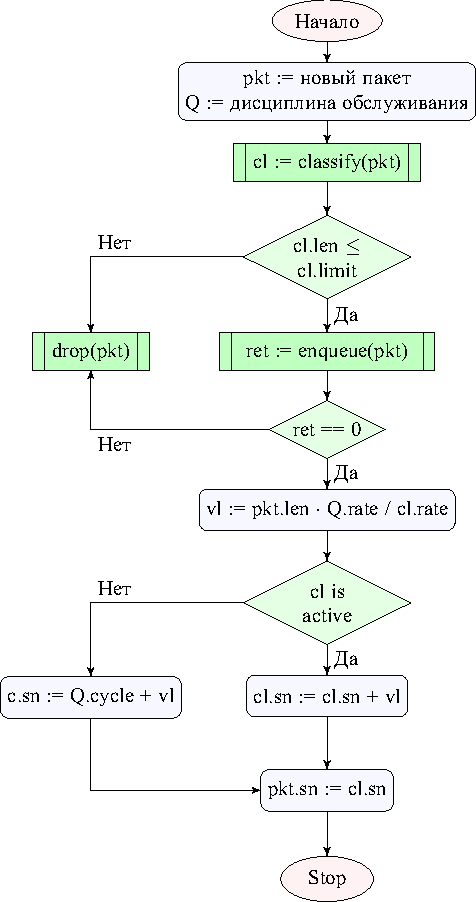
\includegraphics{pdfimages/enq_algo.pdf}
                \caption{Блок-схема алгоритма добавления пакета в очередь.}
        		\label{pic:enqchart}
            \end{figure}

		\subsubsection{Удаление пакета из очереди}

			Функция удаления пакета из очереди непосредственно реализует
			планировщик WFQ.

			\begin{algorithmic}[1]
				\Function{dequeue}{Q}
					%\State {// Находим класс с наименьшим порядковым номером.}
					%\State {// Реализуется это простым простым прохождением по списку}
					%\State {// классов.}
					\State C $\gets$ FIND\_MIN(Q)
					%\State {// Если не найдено классов, то все очереди пусты.}
					\If {C is null}
						\State \Return null
					\EndIf
					\State pkt $\gets$ C.QUEUE.DEQUEUE(C.queue)
					%\State {// Счётчик циклов обновляется после обслуживания пакета;}
					\If {c.queue.len == 0}
					%	\State {// Когда поток становится неактивным, счётчик сбрасывается.}
						\State cl.sn $\gets$ 0
					\EndIf
					\If {все классы не активны}
						\State Q.sn $\gets$ 0
					\Else
    					\State Q.sn $\gets$ pkt.sn
					\EndIf
					\State \Return pkt 
				\EndFunction
			\end{algorithmic}

			В первую очередь в строке 2 находим класс с наименьшим порядковым номером
			пакета в голове очереди. Если класс не был найден, значит все очереди пусты (строка 3),
			и алгоритм не может вернуть пакет. Иначе достаём пакет из очереди (строка 6).
			Проверяем, пуста ли очередь, в строке 8. Если пуста, то класс
			становится неактивным и счётчик сбрасывается (строка 11). В ином случае
			увеличиваем счётчик циклов всей дисциплины в строке 13. И возвращаем
			пакет.
			Блок-схема алгоритма приведена на рисунке~\ref{pic:deqchart}.
			\newpage
            \begin{figure}[ht!]
                \center
                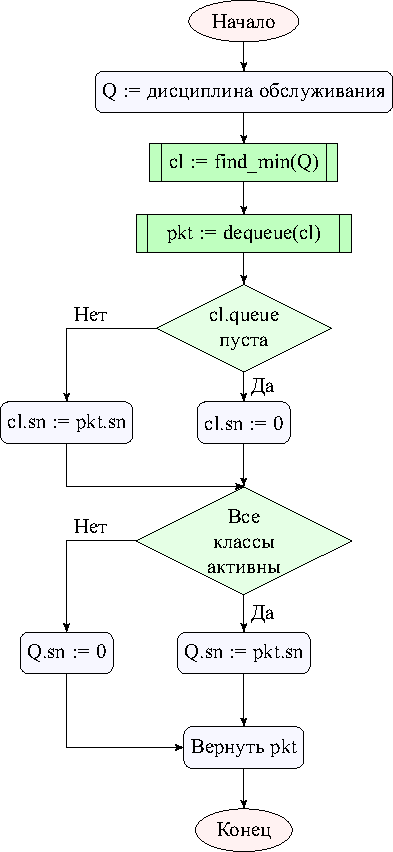
\includegraphics{pdfimages/deq_algo.pdf}
                \caption{Блок-схема алгоритма удаления пакета из очереди.}
        		\label{pic:deqchart}
            \end{figure}
